\documentclass{article}

\usepackage[dutch]{babel}
\usepackage[margin=3cm]{geometry}
\usepackage{graphicx}
\usepackage{float}
\usepackage{caption}
\usepackage{hyperref}
\usepackage{amsmath}
\usepackage{wrapfig}
\usepackage[parfill]{parskip}

% fonts
\usepackage[T1]{fontenc}
\usepackage{helvet}
\renewcommand{\familydefault}{\sfdefault}

\graphicspath{{img/}}
 
\newcommand{\bold}[1]{\textbf{#1}}

\usepackage{minted}
\setminted{frame=single,framesep=3pt,linenos}
\usepackage{upquote}
\usepackage{color}

\begin{document}

\begin{titlepage}
    \author{Tuur Vanhoutte}
    \title{Big Data - Labo}
\end{titlepage}

\pagenumbering{gobble}
\maketitle
\newpage
\tableofcontents
\newpage

\pagenumbering{arabic}

\section{Intro}

Topics:

\begin{itemize}
    \item Linux basics + containers
    \item Elastic search (text search, document store)
    \item Linux Batch Processing \& Dask
    \item InfluxDB (timeseries)
    \item Cloud services (Kafka, Kinesis, Lambda, ML services, \dots)
\end{itemize}

\section{NAT-ing}

\subsection{NAT}

= Network Address Translation

\begin{figure}[H]
    \centering
    \includegraphics[width=0.5\textwidth]{nat.png}
    \caption{NAT diagram}
\end{figure}

\subsubsection{The problem}

\begin{itemize}
    \item We only have one (public/private) IP-address
    \begin{itemize}
        \item Howest: 172.23.82.60
    \end{itemize}
    \item Connecting to a server over a network:
    \begin{itemize}
        \item Using a protocol (HTTP) which uses TCP
        \item Our server has an IP address: 172.23.82.60
        \item Our server is listening at port 5000
        \item $\Rightarrow$ \url{http://172.23.82.60:5000}
    \end{itemize}
    \item Problem: We want to have multiple IP addresses
    \begin{itemize}
        \item Student 1 wants to reach http://192.168.20.21:5000
        \item Student 2 wants to reach http://192.168.20.22:5000
        \item Student x  wants to reach http://192.168.20.xx:5000
    \end{itemize}
\end{itemize}

\subsubsection{The solution}

Translation is needed!

\begin{itemize}
    \item 172.23.82.60:5000 should point to 192.168.20.21:5000
    \item 172.23.82.60:5001 should point to 192.168.20.22:5000
    \item 172.23.82.60:5xxx should point to 192.168.20.xx:5000
\end{itemize}

We can use any port, on both sides:

\begin{itemize}
    \item 172.23.82.60:8000 can point to 192.168.20.21:5000
    \item 172.23.82.60:8000 can point to 192.168.20.21:3000
\end{itemize}

\subsection{SSH Tunnel}

= SSH Port Forwarding

\begin{figure}[H]
    \centering
    \includegraphics[width=0.5\textwidth]{ssh-tunnel.png}
    \caption{Example}
\end{figure}

\begin{figure}[H]
    \centering
    \includegraphics[width=0.7\textwidth]{ssh-tunnel2.png}
    \caption{Voorbeeld: een tunnel wordt opengemaakt en er wordt ingelogd in user@instance}
\end{figure}


\section{Container technology}

\subsection{Docker}

\begin{itemize}
    \item Docker = ecosystem for creating and running containers
    \item Docker wants to make it possible to install and run software on any system
    \item Other reasons: Microservices/DevOps/Resource usage
    \item Docker != Container
    \begin{itemize}
        \item Docker CLI
        \item Docker Engine
        \item Docker Image
        \item Docker Container
        \item Docker Hub
        \item Docker Compose
        \item Docker Swarm
        \item \dots
    \end{itemize}
\end{itemize}

\subsection{Microservices}

\begin{itemize}
    \item = A software development technique
    \item Structure an application as a collection of loosely coupled services
    \item Lightweight
    \item Microservices-based architectures enable continuous delivery and deployment
    \item \url{https://en.wikipedia.org/wiki/Microservices}
\end{itemize}

\subsubsection{Monolithic vs Microservices}

\begin{figure}[H]
    \centering
    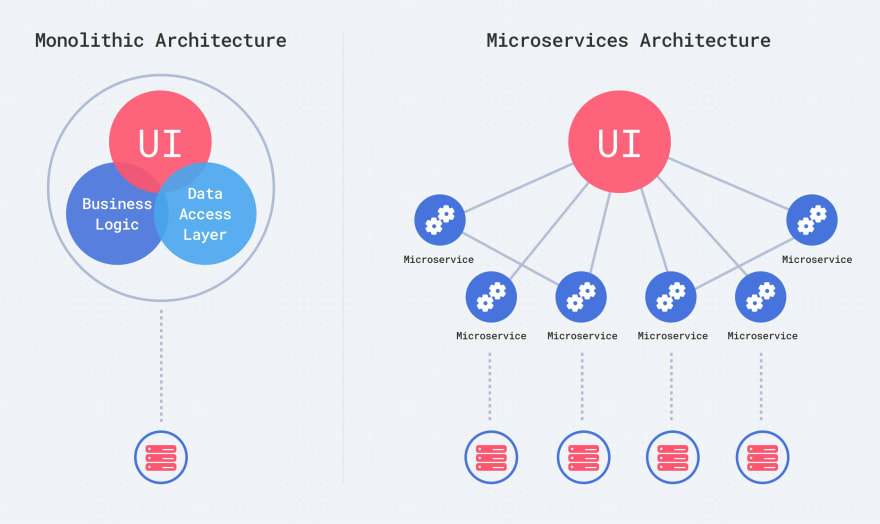
\includegraphics[width=0.5\textwidth]{monolithic-vs-microservices.png}
    \caption{Monolithic architecture vs Microservices architecture}
\end{figure}

\begin{figure}[H]
    \centering
    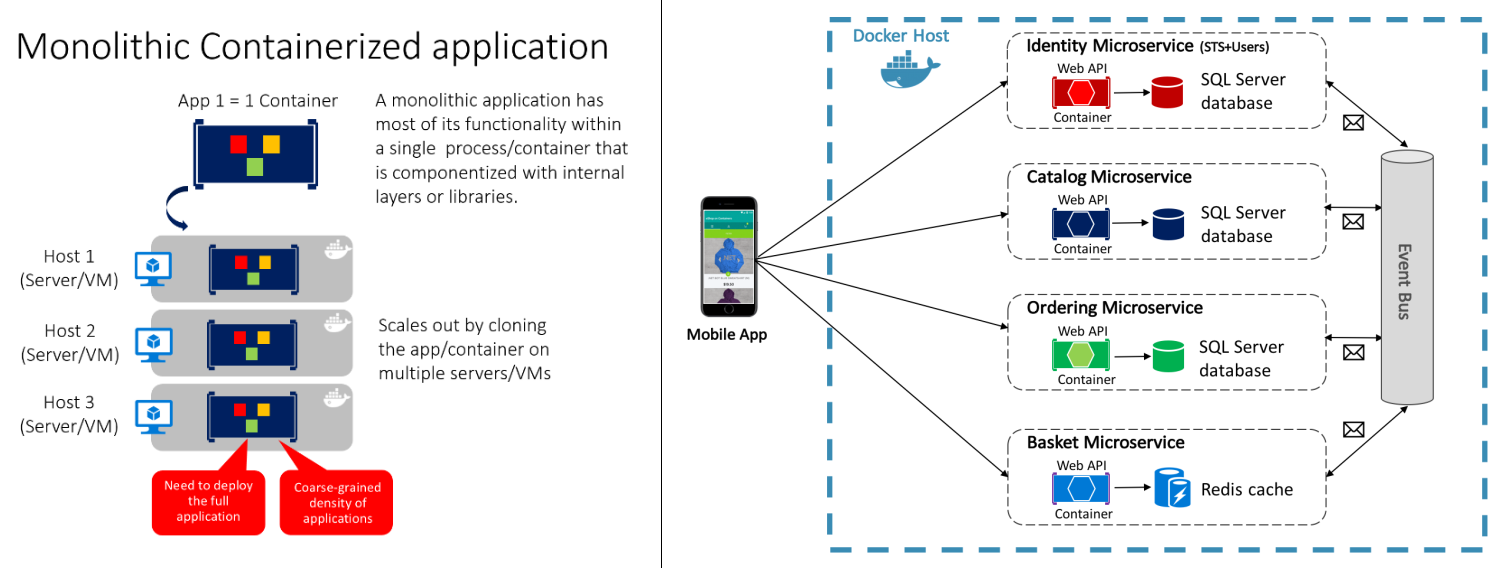
\includegraphics[width=0.5\textwidth]{monolithic-vs-microservices2.png}
    \caption{Monolithic Containerized application}
\end{figure}

Microservices does \bold{not} necessarily mean containerization!

\subsection{Virtualization vs Containerization}

\begin{figure}[H]
    \centering
    \includegraphics[width=0.5\textwidth]{virtualization-vs-containerization.png}
    \caption{Virtualization vs Containerization}
\end{figure}

\subsubsection{Virtualization}

\begin{itemize}
    \item = An abstraction of physical hardware turning one server into many servers
    \item Multiple VMs can run on the same machine
    \item Each VM includes a full copy of an Operating System (OS), one or more apps
    \item Takes a lot of space
    \item Can be slow to boot
\end{itemize}

\subsubsection{Containerization}

\begin{itemize}
    \item = An abstraction at the app layer that packages code and dependencies together
    \item Multiple containers can run on the same machine, they share the OS kernel with each other, each running as isolated processes in user space.
    \item Takes up less space than VMs
    \item Boot up almost instantly
\end{itemize}

\begin{figure}[H]
    \centering
    \includegraphics[width=0.5\textwidth]{virtualization-vs-containerization2.png}
    \caption{Schematic }
\end{figure}

\subsection{Shared kernel}

\subsubsection{What is a kernel?}

\begin{itemize}
    \item Piece of software that offers basic functionality to the OS
    \item System calls: open, read, write, close, wait, exit, \dots
    \item A typical kernel has a few hundred system calls
\end{itemize}

\begin{figure}[H]
    \centering
    \includegraphics[width=0.3\textwidth]{kernel.png}
    \caption{The kernel is the layer that communicates between hardware and applications}
\end{figure}


\begin{itemize}
    \item Docker shares the host OS kernel
    \begin{itemize}
        \item Host OS: Windows / MacOS / Linux
        \item Shared Linux Kernel
    \end{itemize}
\end{itemize}

\begin{figure}[H]
    \centering
    \includegraphics[width=0.5\textwidth]{kernel2.png}
    \caption{Kernel in detail}
\end{figure}

\begin{itemize}
    \item The Ubuntu container requires the Linux kernel
    \item The Linux kernel runs in a Virtual Machine
\end{itemize}

\begin{figure}[H]
    \centering
    \includegraphics[width=0.45\textwidth]{kernel3.png}
    \includegraphics[width=0.45\textwidth]{kernel4.png}
    \caption{}
\end{figure}

\subsubsection{How?}

Two important Linux kernel features:

\begin{itemize}
    \item \bold{Namespaces} are a feature of the Linux kernel that partitions kernel resources
    \item \bold{cgroups} (control croups) is a Linux kernel feature that limits, accounts for, and isolates resource usage of a collection of processes 
\end{itemize}

Simpler:

\begin{itemize}
    \item Namespaces = isolating resources per process (or group of processes)
    \item cgroups = Limitating resource usage per process (or group of processes)
\end{itemize}

\subsubsection{Namespaces}

\begin{itemize}
    \item 7 types:
    \begin{itemize}
        \item mount, UTS, IPC, network, PID, cgroup, user
    \end{itemize} 
    \item For the process (or group of processes) it looks like there is a completely isolated set of resources
\end{itemize}

\subsubsection{Containers}

What is a container?

\begin{itemize}
    \item One or more running processes (if not running anymore $\Rightarrow$ container dead)
    \item Resources are specifically assigned to it
    \item The real bulding blocks: Linux kernel features
    \begin{itemize}
        \item Namespaces
        \item cgroups
    \end{itemize}
\end{itemize}

\subsection{Images}

What is an image?

\begin{itemize}
    \item Filesystem snapshot
    \item Startup command
    \item Layered structure \bold{\textcolor{red}{(!)}}
\end{itemize}

Instance of image = container

\subsubsection{Image layer}

\begin{figure}[H]
    \centering
    \includegraphics[width=0.8\textwidth]{image-layers.png}
    \caption{Image layers}
\end{figure}

\begin{itemize}
    \item RUN, COPY, ADD
    \begin{itemize}
        \item = new read-only layer
    \end{itemize}
    \item Top layer = container layer
    \begin{itemize}
        \item Writeable
    \end{itemize}
    \item Delete container = delete container layer
    \begin{itemize}
        \item Image will still exist
        \item Peristent volumes
    \end{itemize}
\end{itemize}


\subsection{Docker is lightweight}

\begin{itemize}
    \item Shared kernel
    \item Container has no OS
    \item Less disk space $\Rightarrow$ sharing layers
    \item Small community images
    \begin{itemize}
        \item ex: Alpine Linux (small, simple, secure)
    \end{itemize}
    \item Current Docker version is using runC (previously LXC = Linux Containers)
    \begin{itemize}
        \item runC = tooling (written in Go) that makes it possible to create and run containers
        \item runC = CLI to `easily' access kernel features such as cgroups and namespacing
        \item runC = successor of libcontainer (developed by Docker)
        \item Open-sourced $\Rightarrow$ better community
        \item runC implements `Open Container Initiative Runtime Specification'
        \item \url{https://github.com/opencontainers/runtime-spec}
    \end{itemize}
\end{itemize}

Docker is `nothing more' than an ecosystem about creating \& running containers

\subsection{Using Docker}

(see slides 40-55 in \underline{02\_big\_data\_01\_containers.pdf} for basic commands)

\subsubsection{Layers bekijken}

With the command `docker history <image | container id>' you'll get an overview of the layers of an image.

\begin{itemize}
    \item Every RUN, COPY, ADD adds a new read-only \underline{layer}
    \item Make Dockerfile more efficient $\Rightarrow$ create less layers
\end{itemize}

\subsubsection{Make Dockerfile more efficient}

Our Dockerfile, before optimalisation:

\begin{minted}{docker}
FROM python:3.9.1-alpine3.13
WORKDIR '/app'
RUN apk add --no-cache linux-headers g++
RUN pip install Flask # we can replace these two lines by:
RUN pip install uwsgi # RUN pip install -r requirements.txt
COPY ./ ./
RUN addgroup -S uwsgi && adduser -S uwsgi -G uwsgi
USER uwsgi
CMD ["uwsgi", "--ini", "app.ini"]
\end{minted}

After optimalisation:

\begin{minted}{docker}
FROM python:3.9.1-alpine3.13
WORKDIR '/app'
RUN apk add --no-cache linux-headers g++
# the addgroup and adduser commands can be higher up
RUN addgroup -S uwsgi && adduser -S uwsgi -G uwsgi
# first, we copy the requirements.txt file
COPY ./requirements.txt ./
# then we install ALL packages
RUN pip install -r requirements.txt
# then we copy the remaining files
COPY ./ ./
USER uwsgi
CMD ["uwsgi", "--ini", "app.ini"]
\end{minted}

\subsubsection{Connecting to a database in a different container}

Use `ip a' to find the correct ip to use in this command:

\begin{minted}{bash}
docker run -p 8080:8080 
    -e POSTGRES_PASSWORD=student_password 
    -e POSTGRES_USER=student_user 
    -e POSTGRES_DATABASE=labo 
    -e POSTGRES_PORT=5432 
    -e POSTGRES_HOST=ip-van-je-vm  # change this ip
    -e PORT=8080 
    jouw-naam/api                  # change this
\end{minted}

\section{Sharding}

\begin{itemize}
    \item Index = collection of documents
    \item Document = data in JSON format
    \item Shard = A piece of an index. Index is "sharded"\ in blocks, a block = shard
    \item Primary shard = Document is primarily indexed (written) to a primary shard
    \item Replica shard = an asynchronous copy of the primary shard
\end{itemize}

\subsection{Create index}

\begin{minted}{json}
{
    "settings": {
        "number_of_shards": 2,
        "number_of_replicas": 1
    }
}
\end{minted}

How many shards in total: \textbf{4}

\begin{figure}[H]
    \centering
    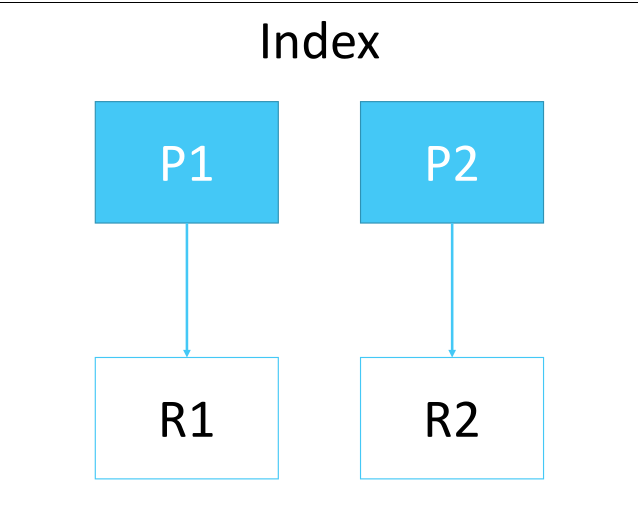
\includegraphics[width=0.3\textwidth]{number-of-shards.png}
    \caption{4 shards: 2 primary shards with 1 replica each}
\end{figure}

\subsection{Health}

Health exists at shard, index and cluster level!

\subsubsection{Shard health}

\begin{itemize}
    \item Green = all shards are allocated
    \item Yellow = all primaries are allocated but at least one replica is not
    \item Red = at least one primary shard is not allocated in the cluster
\end{itemize}

\subsubsection{Index health}

= status of the worst shard in that index

\subsubsection{Cluster health}

= status of the worst index in the cluster

\subsection{Shard allocation}

Shards states:

\begin{itemize}
    \item Unassigned = master did not assign the shard (yet)
    \begin{itemize}
        \item Or master is not able to assign the shard
    \end{itemize}
    \item Initializing = master did assign the shard, creating\dots
    \item Started = shard is fully operational
    \item Relocating = shard is moving
    \begin{itemize}
        \item Imbalance, new nodes, removed nodes, \dots
    \end{itemize}
\end{itemize}

\subsubsection{Unassigned}

\begin{figure}[H]
    \centering
    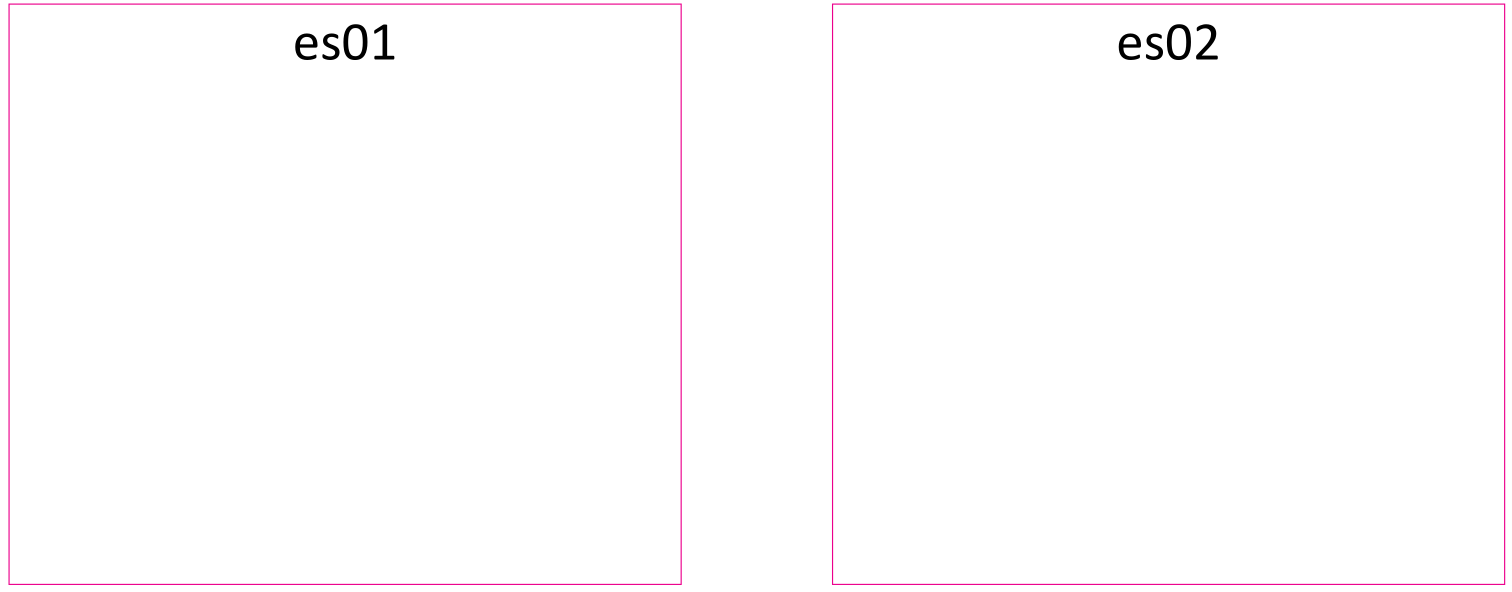
\includegraphics[width=0.5\textwidth]{shard-alloc-unassigned.png}
    \caption{No shards assigned yet}
\end{figure}

\subsubsection{Initializing}

\begin{figure}[H]
    \centering
    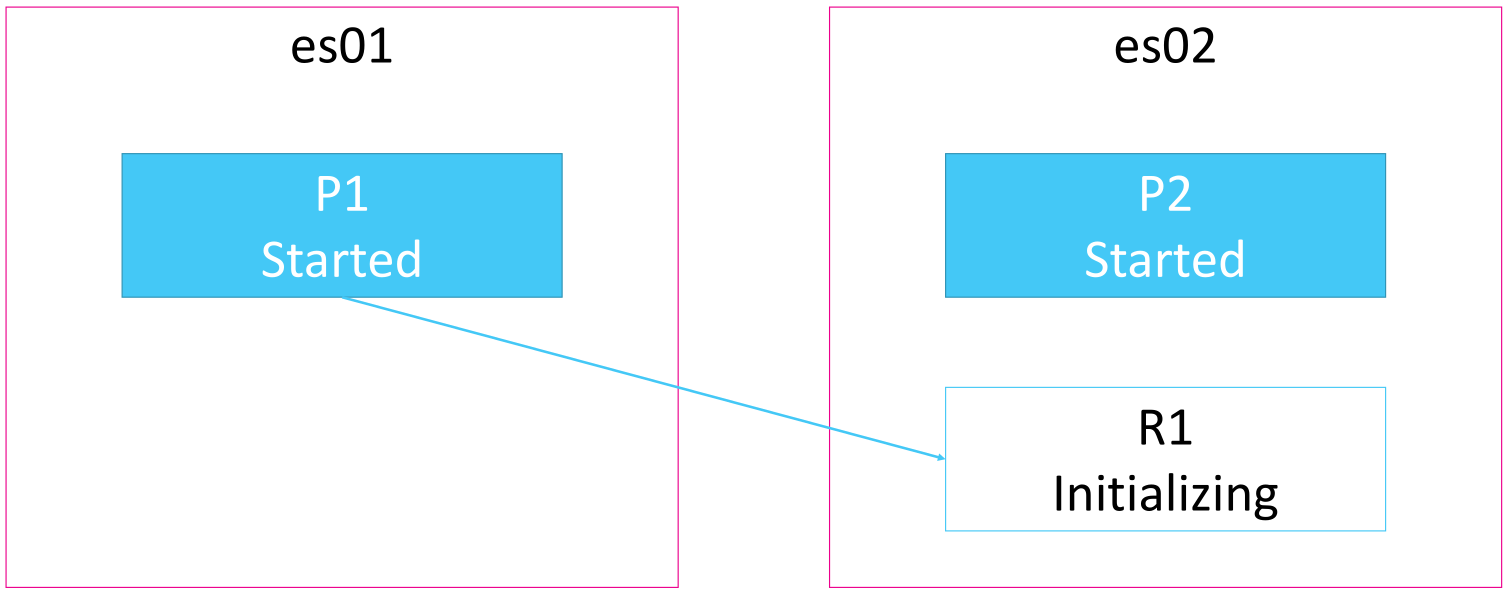
\includegraphics[width=0.5\textwidth]{shard-alloc-initializing.png}
    \caption{Creating shards}
\end{figure}

\subsubsection{Started}

\begin{figure}[H]
    \centering
    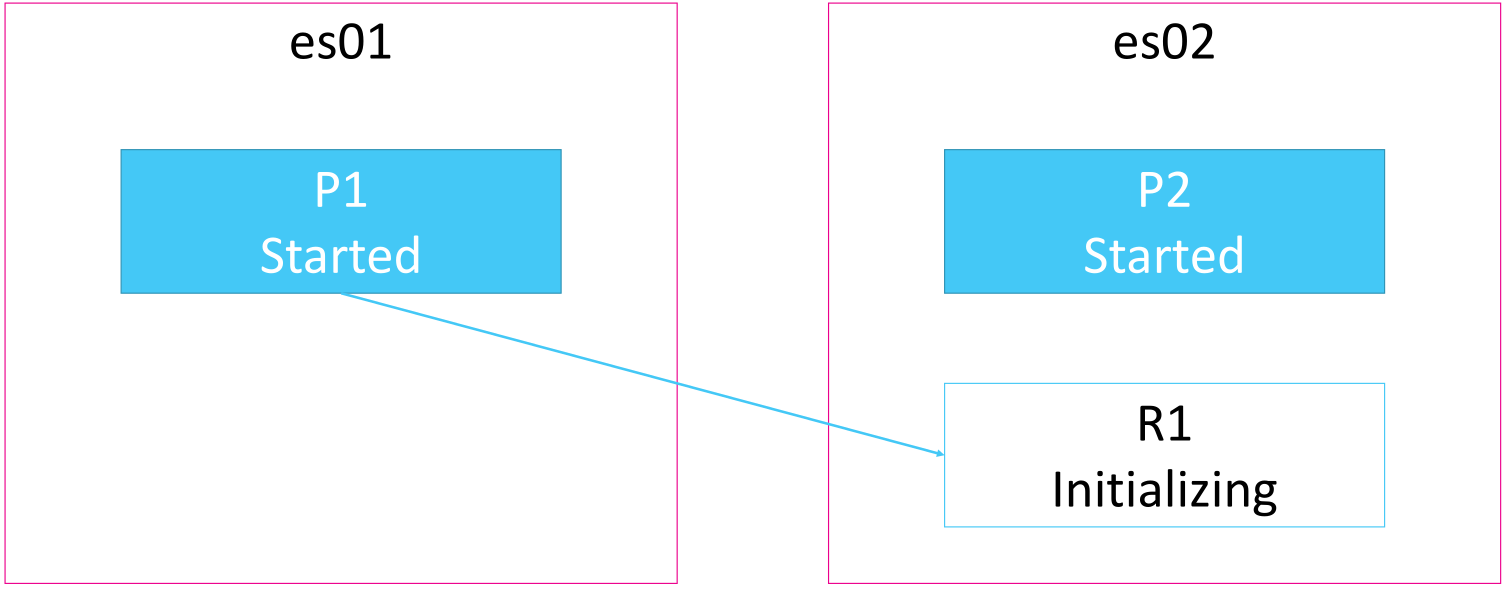
\includegraphics[width=0.5\textwidth]{shard-alloc-started.png}
    \caption{The primary shards have been started, replica 1 is initializing. \textbf{Cluster status = yellow}}
\end{figure}
\begin{figure}[H]
    \centering
    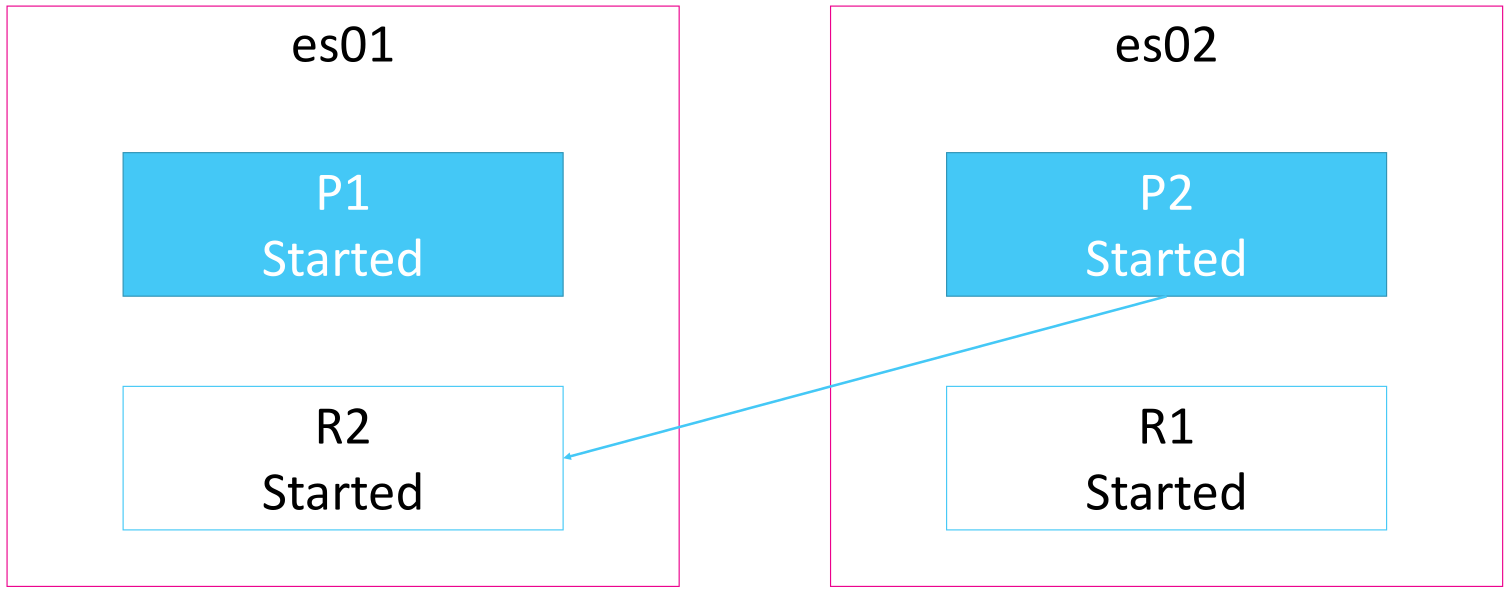
\includegraphics[width=0.5\textwidth]{shard-alloc-started2.png}
    \caption{\textbf{Cluster status = green}}
\end{figure}

\textbf{What if one of the node fails?}

\begin{figure}[H]
    \centering
    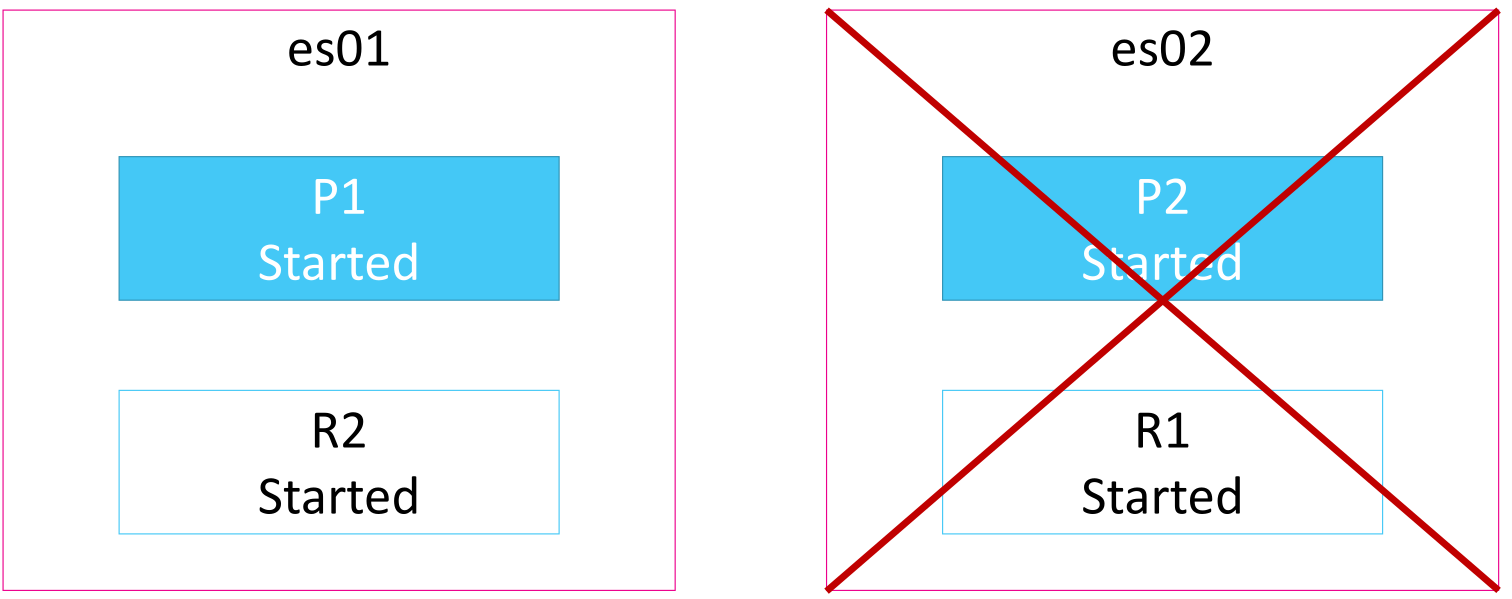
\includegraphics[width=0.5\textwidth]{shard-alloc-started3.png}
    \caption{Situation when one node fails}
\end{figure}
\begin{figure}[H]
    \centering
    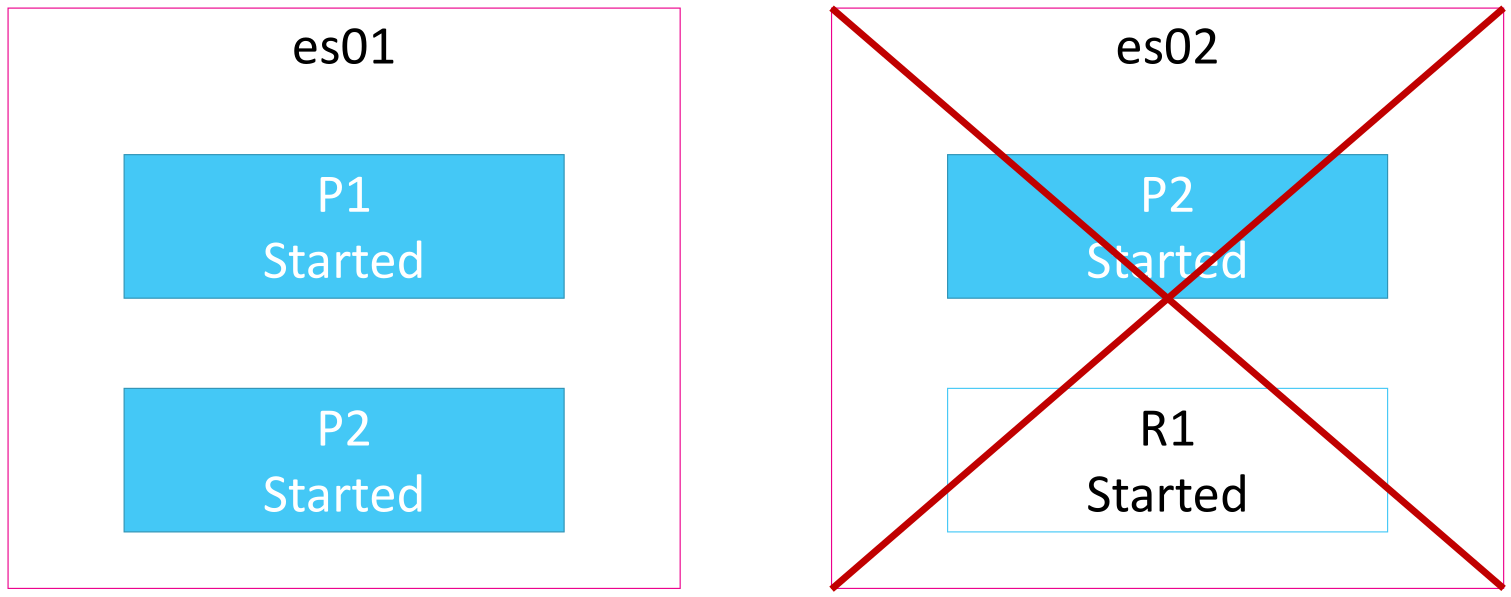
\includegraphics[width=0.5\textwidth]{shard-alloc-started4.png}
    \caption{After some time, R2 will become a primary shard. \textbf{Cluster status = yellow}}
\end{figure}

\subsubsection{Relocating}

\begin{figure}[H]
    \centering
    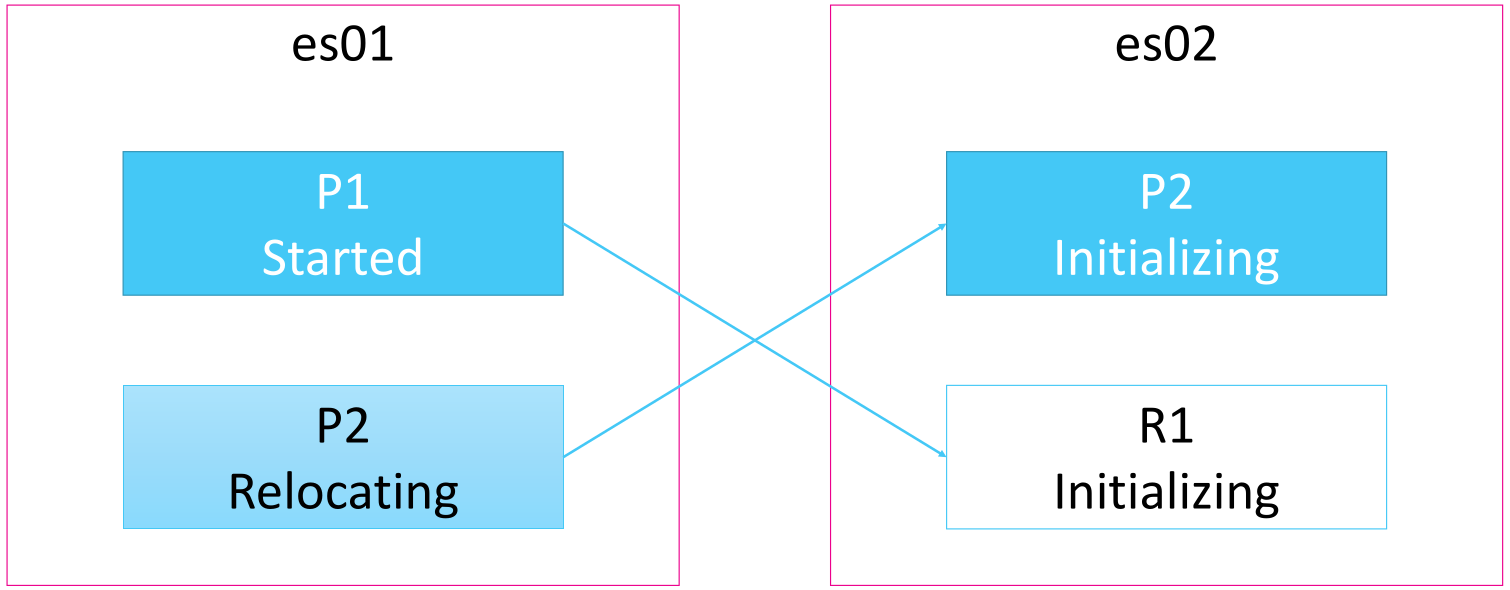
\includegraphics[width=0.5\textwidth]{shard-alloc-relocating.png}
    \caption{After es02 is restored, P2 gets relocated to its previous node}
\end{figure}

\subsection{Change number of replicas}

\begin{minted}{json}
{
    "index": {
        "number_of_replicas": 0
    }
}
\end{minted}

How many shards in total? \textbf{2}

\begin{figure}[H]
    \centering
    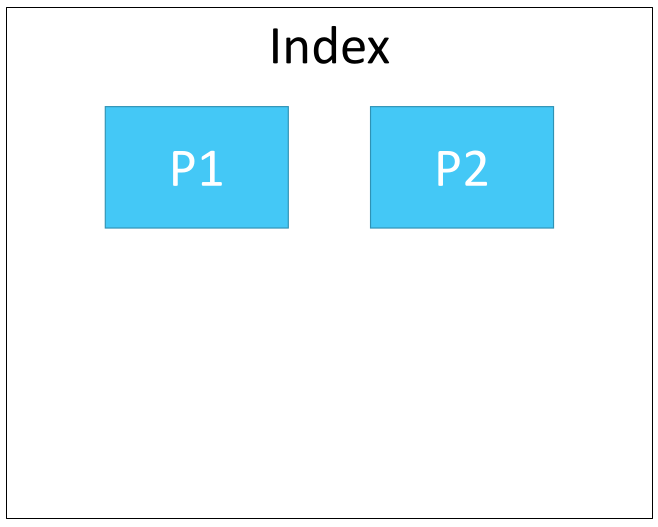
\includegraphics[width=0.3\textwidth]{change-number-of-replicas.png}
    \caption{2 shards total: 2 primary shards, 0 replicas each}
\end{figure}

\subsubsection{Health when one fails}

\begin{figure}[H]
    \centering
    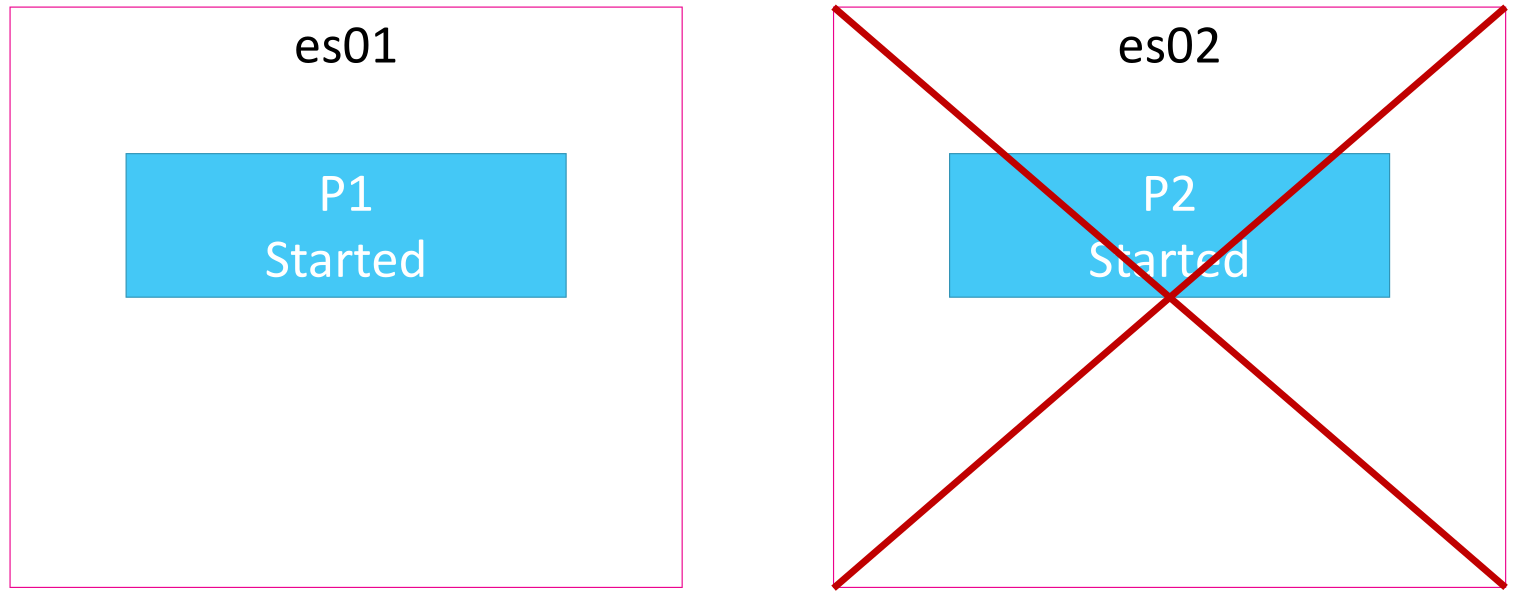
\includegraphics[width=0.5\textwidth]{change-number-of-replicas-red.png}
    \caption{\textbf{Cluster status = Red}}
\end{figure}

\subsection{Caveat: single node cluster}

\begin{itemize}
    \item Bootstrap checks = important settings are checked
    \item discovery.type=single-node
    \item If a node is already part of a cluster:
    \begin{itemize}
        \item Unique node ID
        \item Unique cluster ID
        \item Not easy to create a new cluster
    \end{itemize}
\end{itemize}

\section{Linux batching + Dask}

\subsection{Python \& data engineering/science}

\begin{itemize}
    \item Veel tools, libraries (numpy, pandas)
    \item Jammer genoeg slecht schaalbaar $\Rightarrow$ parallellisatie
    \item Threads/processes kan, maar complex en niet ideaal
    \item Wat als he tniet in memory past?
    \begin{itemize}
        \item Naar disk?
        \item Kan, maar complex! Sommige operaties `vereisen' alles in memory
    \end{itemize}
\end{itemize}

\subsection{Spark vs Dask}
\subsubsection{Spark}

\begin{itemize}
    \item Complex, leercurve!
    \item Complete `engine', clustering
    \item Streaming engine
    \item In Java geschreven: gebruikt de Java Virtual Machine (JVM) $\Rightarrow$ minder toegankelijk
    \item Standalone
\end{itemize}

\subsubsection{Dask}

\begin{itemize}
    \item Eenvoudiger (zeker als je Python kent)
    \item Lightweight, zelfs op 1 node zinnig
    \item Flexibeler, maar minder performant
    \item Integratie met andere libraries
    \item In zekere zin `de Python versie van Spark'
\end{itemize}

\section{TICK Stack}

The Tick stack is an acronym for a platform of open source tools 
built to make collection, storage, graphing, and alerting on 
time series data incredibly easy.

The tools:

\begin{itemize}
    \item Telegraf
    \item InfluxDB
    \item Chronograf
    \item Kapacitor
\end{itemize}


\begin{figure}[H]
    \centering
    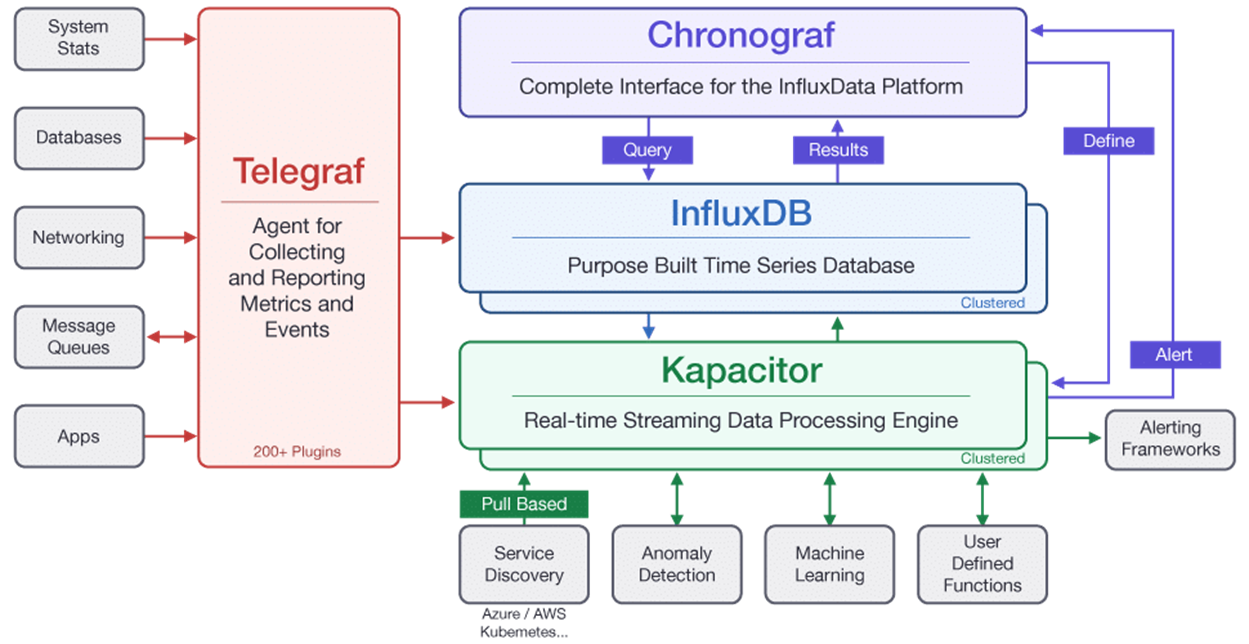
\includegraphics[width=0.5\textwidth]{tick-stack-components.png}
    \caption{The components of the TICK Stack}
\end{figure}

\subsection{Telegraf}

\begin{itemize}
    \item = Agent for collecting and reporting metrics and events
    \item Has inputs and outputs
\end{itemize}

\subsection{InfluxDB}

= Purpose built time series database

\begin{itemize}
    \item Open source
    \item Simple HTTP API (POST, GET) with client libraries
    \item Somewhat similar to classic SQL, there are two versions:
    \begin{itemize}
        \item V1: SQL \& Flux: SELECT * FROM measurement WHERE tag=value
        \item V2: Flux, less like SQL, better for time series data:
\begin{minted}{bash}
# Flux
from(bucket: "bucket")
|> range(start: v.timeRangeStart, stop: v.timeRangeStop)
|> filter(fn: (r) => r["_measurement"] == "test")
\end{minted}
    \end{itemize}
\end{itemize}

\subsubsection{Key concepts}


\begin{itemize}
    \item Line protocol = a text-based format that provides the measurement, tag set, field set, and timestamp of a data point:
\begin{minted}{bash}
weather,location=us-midwest temperature=79,humidity=49 1591711854359    
weather,location=us-midwest temperature=82,humidity=50 1591711787540   
    |    -------------------- --------------------------  |
    |             |             |                         |
    |             |             |                         |
+-----------+--------+-+---------+--------------+---------+
|measurement|,tag_set| |field_set|              |timestamp|
+-----------+--------+-+---------+--------------+---------+
\end{minted}
    \item Measurement = data that belongs together
    \item Timestamp = UNIX format
    \item Tags / Fields = key:value
    \item Tag = metadata
    \begin{itemize}
        \item Tags are indexed
        \item `Fields' where you want to query on
        \item Only strings!
    \end{itemize}
    \item Field = data
    \begin{itemize}
        \item Fields are not indexed
        \item Floats, integers, strings, and booleans
    \end{itemize}
    \item Tag set = set of tags
    \item Field set = set of fields
\end{itemize}

\subsection{Chronograf}

= A visualization tool

\begin{figure}[H]
    \centering
    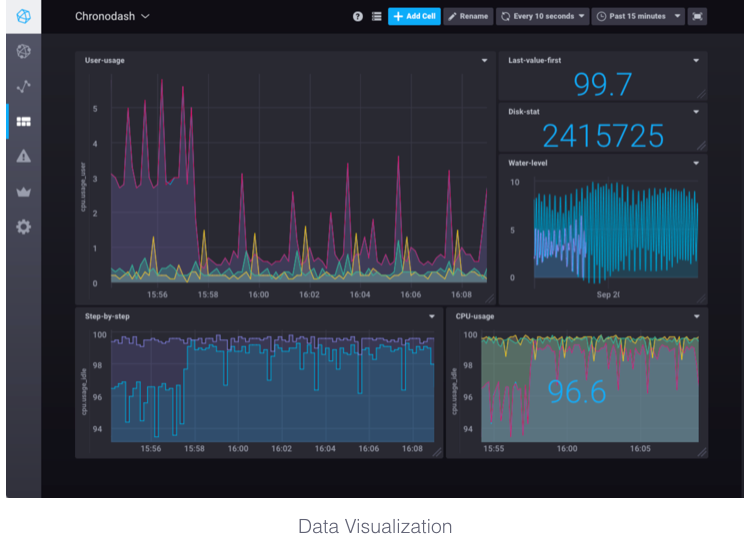
\includegraphics[width=0.45\textwidth]{chronograf-data-visualization.png}
    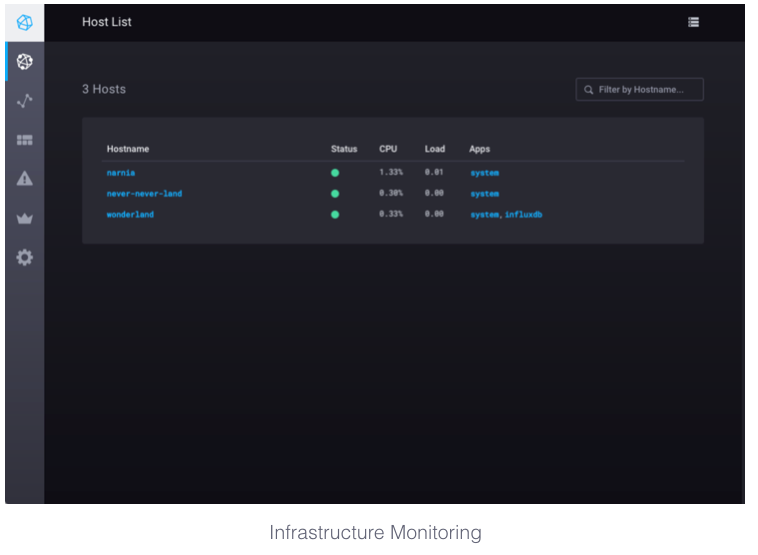
\includegraphics[width=0.45\textwidth]{chronograf-infrastructure-monitoring.png}
    \caption{Data visualization and Infrastructure Monitoring}
\end{figure}

\begin{figure}[H]
    \centering
    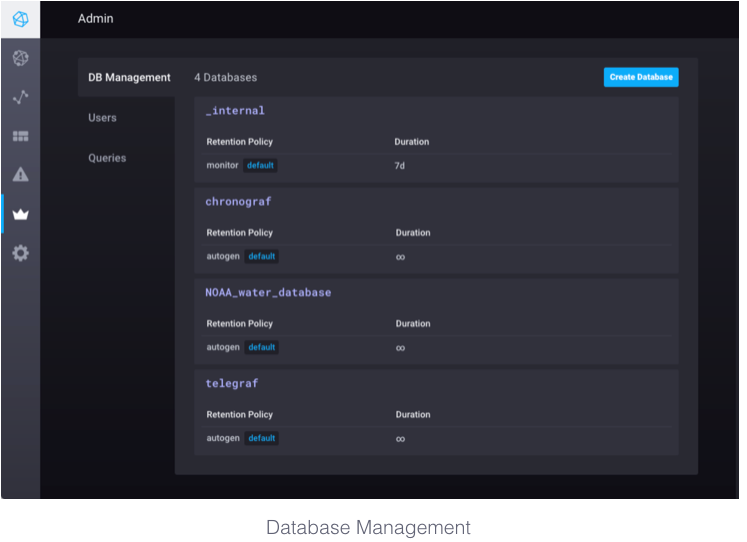
\includegraphics[width=0.45\textwidth]{chronograf-database-management.png}
    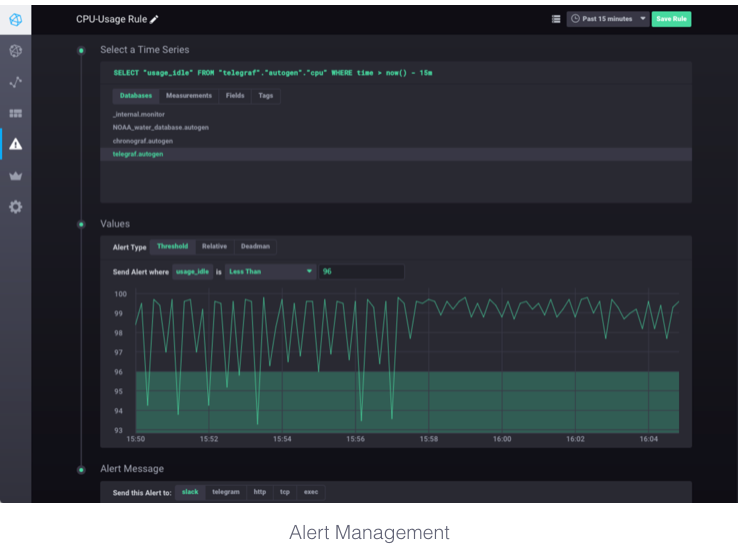
\includegraphics[width=0.45\textwidth]{chronograf-alert-management.png}
    \caption{Database management and alert management}
\end{figure}

\subsection{Kapacitor}

\begin{figure}[H]
    \centering
    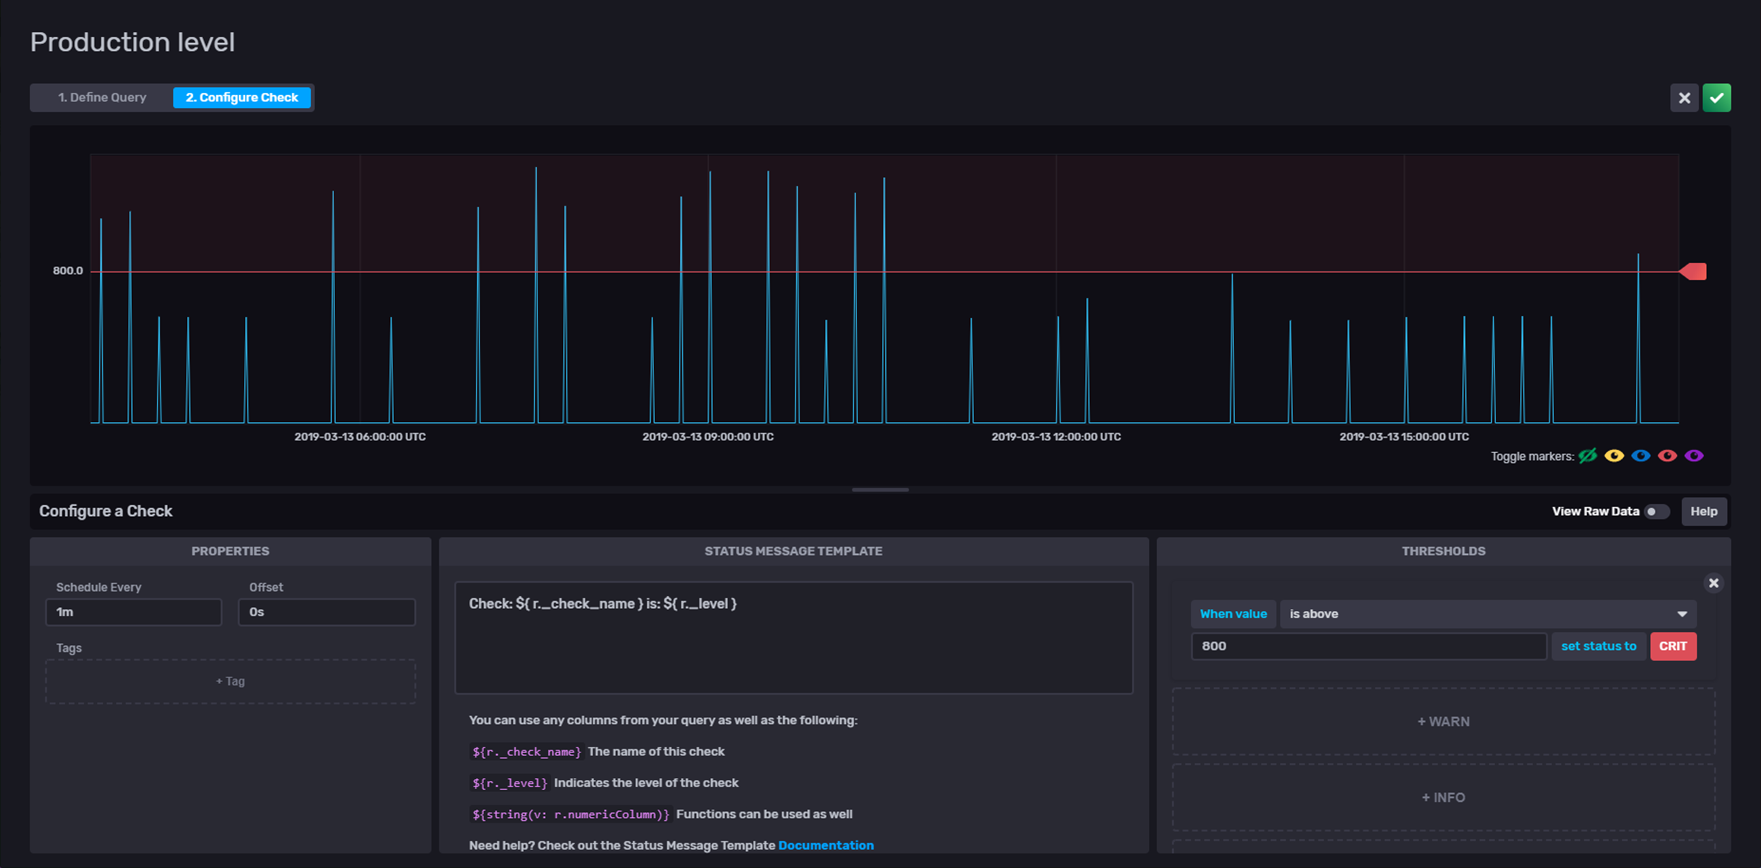
\includegraphics[width=0.5\textwidth]{kapacitor.png}
    \caption{}
\end{figure}

\subsection{Deployment models}

V2

\begin{itemize}
    \item Open source version (OSS)
    \begin{itemize}
        \item No clustering
        \item No out-of-the-box replication
    \end{itemize}
    \item Enterprise version: expensive, contact sales
    \item Cloud version: cheaper, usage based
    \item Chronograf and InfluxDB: one component
    \item Multi-tenant focus
\end{itemize}

\begin{figure}[H]
    \centering
    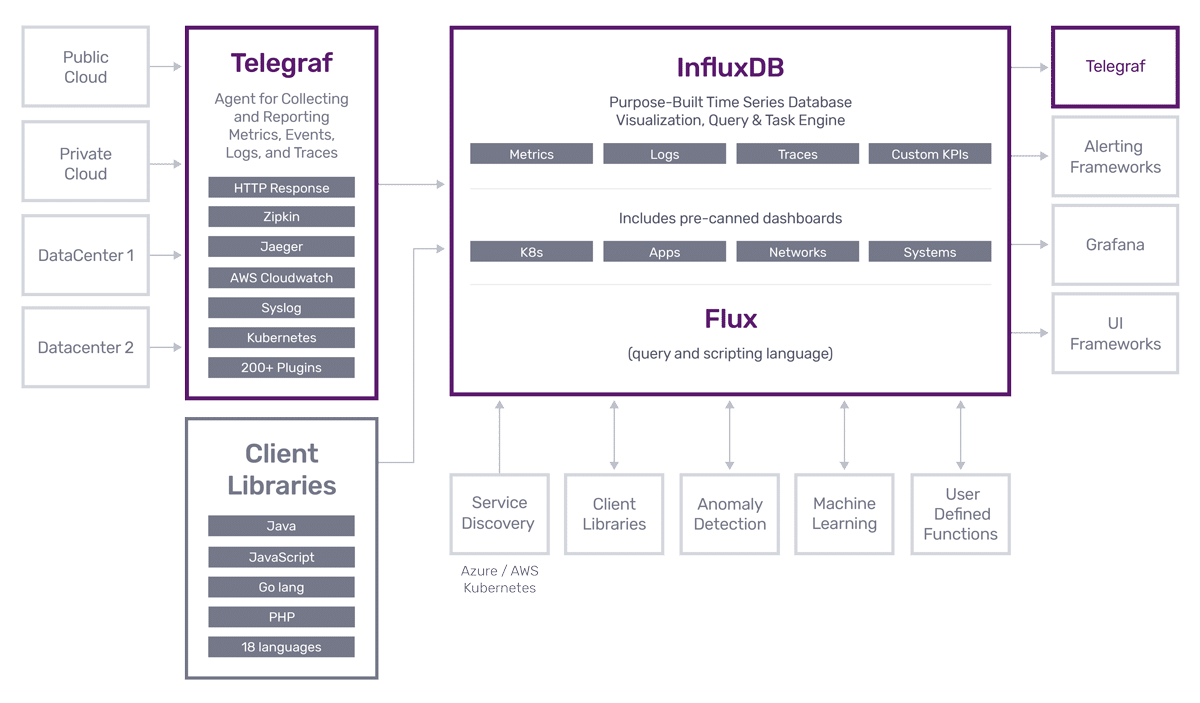
\includegraphics[width=0.5\textwidth]{influxdb-2.png}
    \caption{InfluxDB 2.0: a better graphic}
\end{figure}

\subsection{Architecture of the TICK stack}

\subsubsection{Write Ahead Log (WAL)}

\begin{figure}[H]
    \centering
    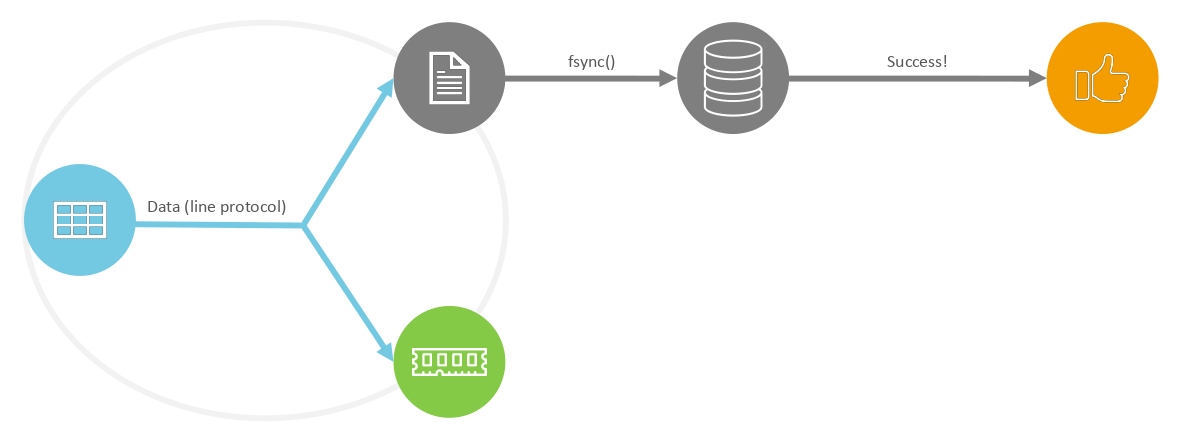
\includegraphics[width=0.5\textwidth]{tick-architecture-wal.png}
\end{figure}

\begin{itemize}
    \item Disk optimized format (fast writes $\leftrightarrow$ slow queries)
    \begin{itemize}
        \item Not optimized for fast queries $\Rightarrow$ memory!
    \end{itemize}
    \item In case of a crash: replay WAL (durability $\uparrow$)
    \item What if we have more data than memory?
    \begin{itemize}
        \item Out-of-memory errors (OOM)
    \end{itemize}
    \item InfluxDB v1 vs v2  \& OSS vs cloud:
    \begin{itemize}
        \item V1 \& V2 OSS: flat, simple file
        \item V2 cloud: Kafka
    \end{itemize}
\end{itemize}

\subsubsection{Time Structured Merge Tree (TSM)}

\begin{itemize}
    \item A data structure optimized for storage and fast time-series queries
    \item Compressed data in columnar format
    \item Easy memory-mapping
    \item Similar to Log Structured Merge Tree (LSM)
    \item Field values are grouped by series key, ordered by time
    \item Series key = measurement, tag set and (a single) field key
\end{itemize}

\begin{figure}[H]
    \centering
    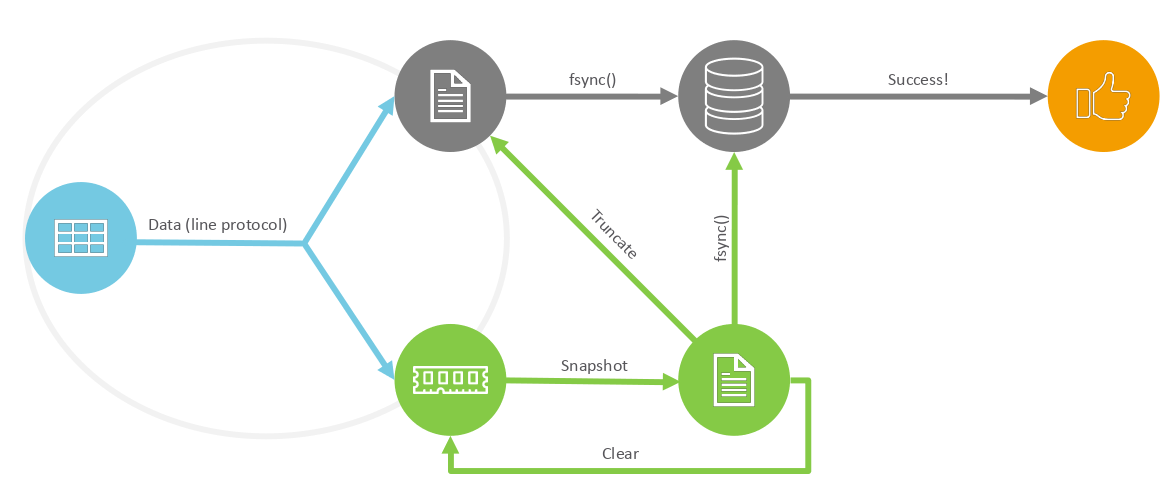
\includegraphics[width=0.5\textwidth]{tick-architecture-wal-tsm.png}
    \caption{TSM + WAL}
\end{figure}

\begin{itemize}
    \item Fast(er) queries: only read required series
    \item Compression: saved data is smaller than original (more data per node)
    \item Columnar: easy for memory-mapping
    \begin{itemize}
        \item Data is cached for a limited time (solves OOM)
    \end{itemize}
    \item What if we have many series keys (high cardinality)
    \begin{itemize}
        \item Finding the right data will be slow!
    \end{itemize}
\end{itemize}

\subsubsection{Time series index (TSI)}

\begin{itemize}
    \item A data structure optimized for storage and fast query of series keys
    \begin{itemize}
        \item TSM stores the data grouped by the series key
        \item TSI stores the series keys grouped by measurement, tag and field key
    \end{itemize}
    \item TSI answers two questions:
    \begin{itemize}
        \item What measurements, tags and fields exists?
        \item Given a measurement, tag, field, what series key exists?
    \end{itemize}
    \item TSI stores the index in memory and on disk
    \begin{itemize}
        \item Memory = page cache (least recently used memory)
        \item Disk: writes to a WAL, compaction in the background
    \end{itemize}
\end{itemize}

\subsubsection{Sharding}

V1:

\begin{itemize}
    \item Directory with WAL, TSM and TSI files
    \item Retention policy (on database level)
    \item Each shard has a start and endtime
    \item Scalability \dots but only for InfluxDB Cloud / InfluxDB Enterprise
\end{itemize}

V2:

\begin{itemize}
    \item Sharding in V1 has much overhead: WAL, TSM and TSI / shard 
    \begin{itemize}
        \item Too much redundant data, especially for the TSI
        \item Too many writes
    \end{itemize}
    \item Not everyone needs a retention policy
    \item Sharding is now implemented as a block, like in most other database systems (in OSS only 1 shard)
\end{itemize}

\subsection{Pitfalls, tips \& tricks}

\begin{itemize}
    \item Tips for optimal (write) performance:
    \begin{itemize}
        \item Order your timestamps
        \item Order your tags alphabetically
        \item Use the right precision: seconds, milliseconds, microseconds or nanoseconds
        \item Write in bulks (less fsync's)
    \end{itemize}
    \item Duplicates: measurement, tag set \& timestamp
    \item Tags vs. Fields 
    \item V2 is a great product, but:
    \begin{itemize}
        \item Documentation is far from complete
        \item Bugs in client libraries, e.g. precision is neglected
        \item Quick release cycle / bug fixes
    \end{itemize}
    \item V1 vs. V2, OSS vs. Cloud vs. Enterprise
\end{itemize}


\end{document}